\documentclass[11pt]{article}
\usepackage{amsmath}
\usepackage{amssymb}
\usepackage{amsthm}
\usepackage{array}
\usepackage{color}
\usepackage{lmodern}
\usepackage{hyperref}

\usepackage{graphicx}
\usepackage{algorithm}
\usepackage[noend]{algpseudocode}
\graphicspath{ {./images/} }
\usepackage{xy}
\usepackage[margin=0.9in]{geometry}
\usepackage{verbatim}
\parindent 0in

\usepackage{tikz}

\title{MST and Union Find}
\author{Neeyanth Kopparapu}
\date{October 2019}

\begin{document}
\algrenewcommand{\Return}{\State\algorithmicreturn~}
\maketitle

\section{Introduction - The Problem}
    Suppose we have a set of trees, something we call a \textit{forest}. \footnote{If you don't know what a tree is, go to the other lecture.} We want to know if two nodes are part of the same component. 

\begin{figure}[!hb]
    \centering
    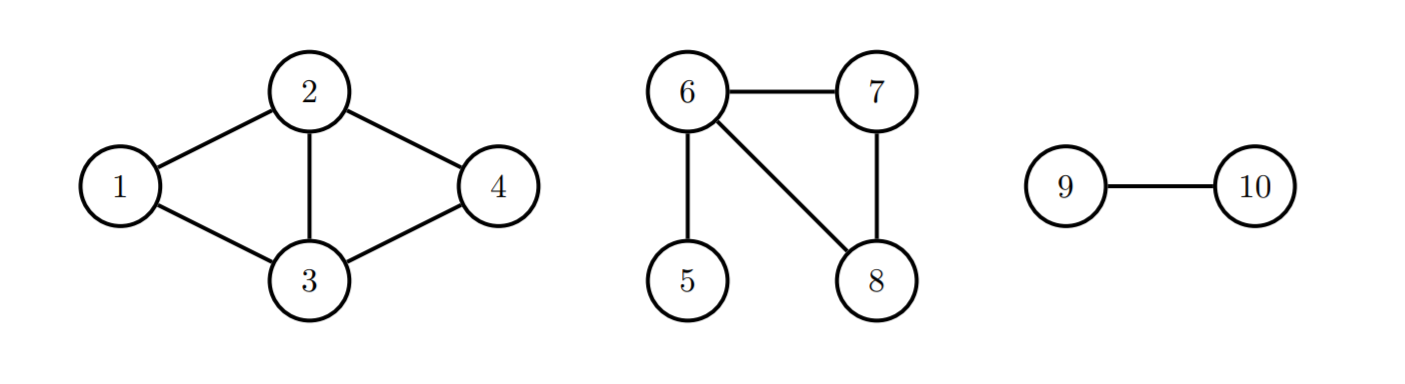
\includegraphics[]{images/graph.png}
    \caption{Your Typical Graph}
    \label{fig:g1}
\end{figure}

    We would do this in the following way:
\begin{itemize}
    \item \textit{find(node)} would give us the \textbf{label} of the component that it belonged to. (This is all we would need if the graph didn't change)
    \item \textit{union($n_1$, $n_1$)} connect the components that contain $n_1$ and $n_2$ and would have the same label.
\end{itemize}

    We are gonna go through some ways to optimize the performance of this and some applications.
\pagebreak
\section{Union Find}
\subsection{Naive Solutions}
We would first think of two solutions:

\subsubsection{Pointer Representation}
    In a graph, keep pointers to parents of nodes. (Arbitrarily choose parents)

\begin{figure}[!hb]
    \centering
    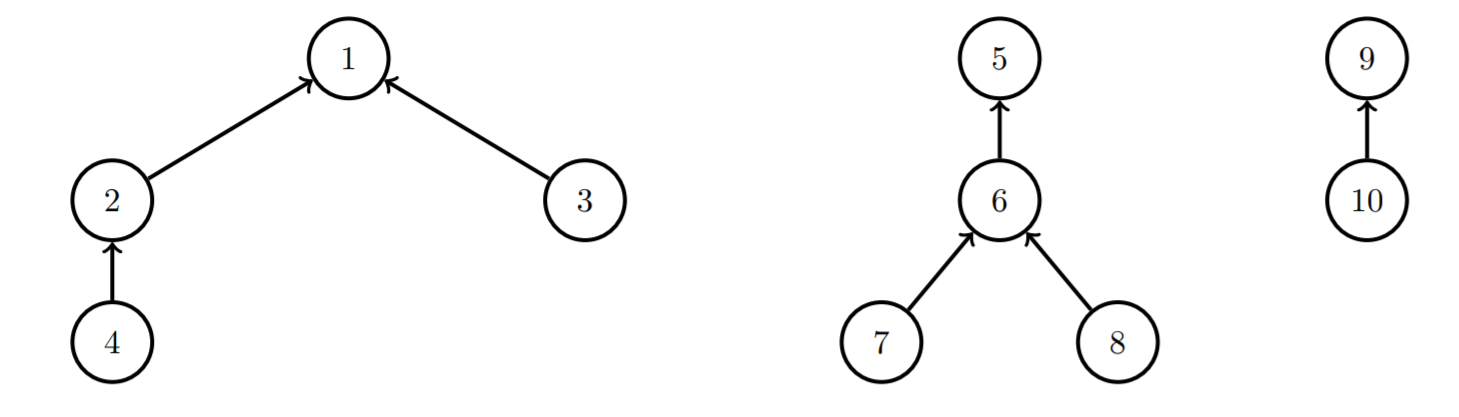
\includegraphics[]{images/digraph.png}
    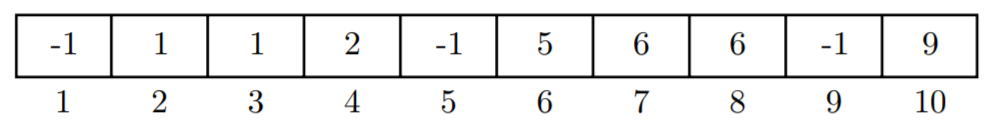
\includegraphics[]{images/pointer.png}
    \caption{Your Typical Graph}
    \label{fig:g1}
\end{figure}
    We can then get \textit{find} by keep tracing parents until we get to $-1$, implying we hit the parent node of the component. \textbf{Question:} What is \textit{find(8)}? Which nodes did you have to trace to get there? \\

    Doing the union is also really easy. If we had to do \textit{union(3,6)}, all we essentially have to do is set the \textit{find} of the root of $3$ to the \textit{find} of $6$. \textbf{Why does this work?} \\
    
    However, we run into a problem - \textit{find} starts to grow linearly. This is a problem in our runtime, we are going for approximately \textbf{constant} complexity. 

\subsubsection{List Representation}
    In a typical graph, we just store (in an array) the label given the vertex. Clearly \textit{find} is linear, but this also makes \textit{union} become linear. \textbf{Why?}
    
\subsection{Optimizations}
    We are going to go back to the pointer representation, because that is what we will optimize. We can make two fixes:
    
    \begin{itemize}
        \item The first is to always add the shorter tree to the taller tree, as we want to minimize the maximum height. An easy heuristic for the height of the tree is simply the number of elements in that tree. We can keep track of the size of the tree with a second array.
        \item The second is a bit more tricky. Assign the pointer associated with \textit{node} to be \textit{find(node)} at the end of the find operation. We can design \textit{find(node)} to recursively call \textit{find} on the pointer associated with \textit{node}, so this fix sets pointers associated with nodes along the entire chain from \textit{node} to \textit{find(node)} to be \textit{find(node)}. 
    \end{itemize}
    
    It turns out that these two optimizations turn the run-time of both operations to $O(\alpha(V))$, where $\alpha(V)$ is the inverse Ackerman function, and for all intensive purposes $\alpha(V) \leq 5$, so this makes is approximately constant. 
    
    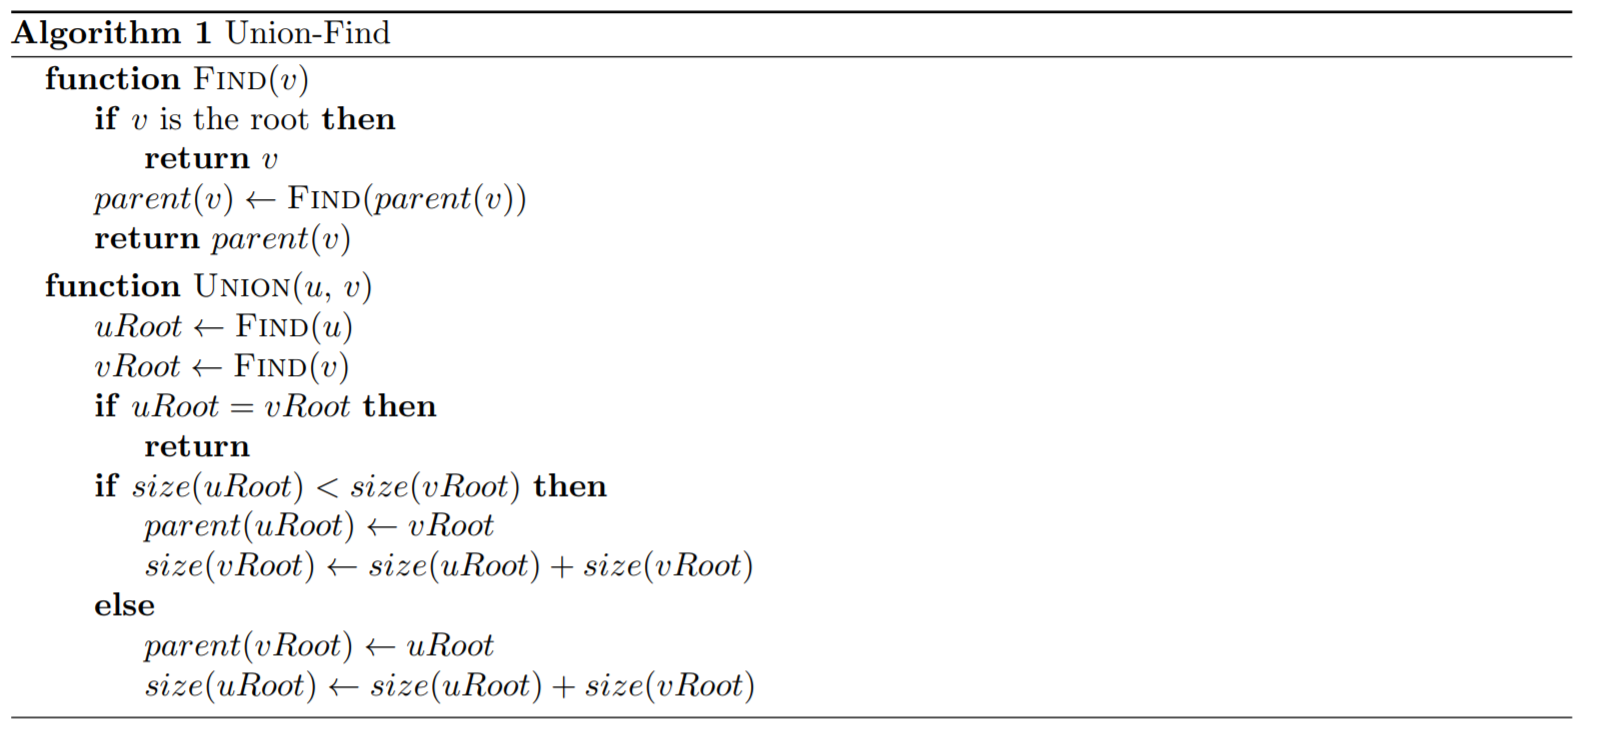
\includegraphics[]{images/UFind.PNG}
    
    With that, we can start with its applications!

\section{Minimum Spanning Tree}

    Consider a connected, undirected graph. A \textit{spanning tree} is a subgraph that is a tree and contains every vertex in the original graph. A \textit{minimum spanning tree} is a spanning tree such that the sum of the edge weights of the tree is minimized. Finding the minimum spanning tree uses many of the same ideas discussed earlier.
    
    \begin{center}
    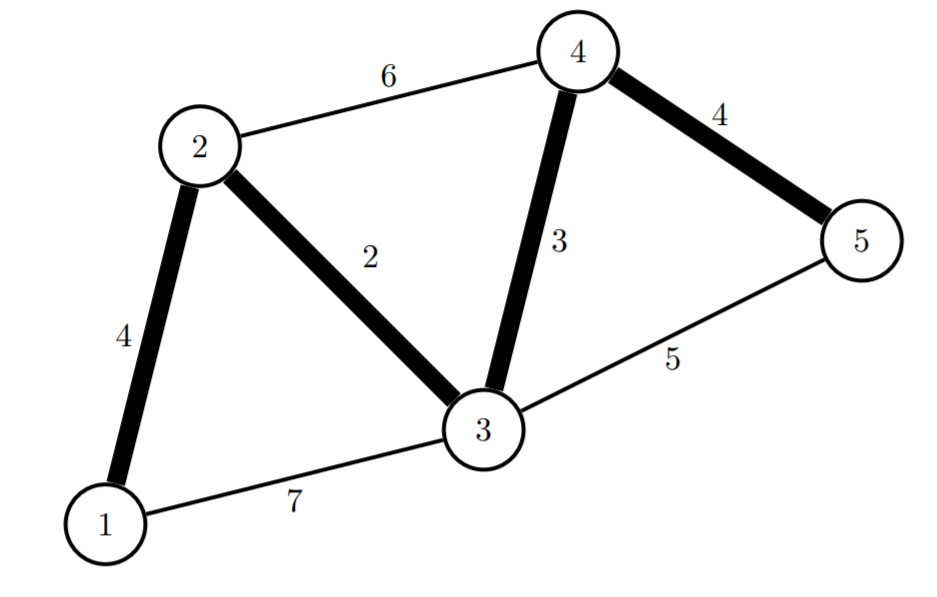
\includegraphics[]{images/MST.png}
    \end{center}
    
    I won't discuss \textbf{Prim's Algorithm} but it is a way to do this. Instead, we are going to talk about \textbf{Kruskal's Algorithm}, essentially an HC of Union-Find in this application. \\
    
    First, we need to sort the edges. Kruskal's algorithm greedy selectes edges that would contribute to the MST until all the nodes are accounted for. Union-Find is the perfect way to make sure all the nodes are accounted for!!
    
    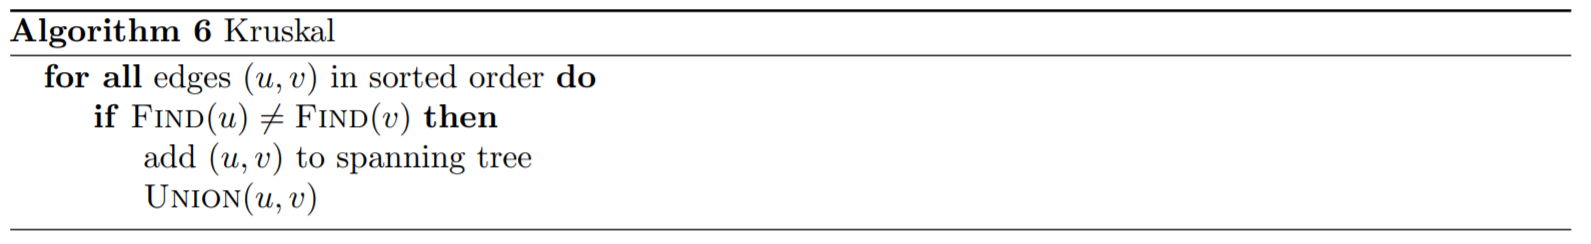
\includegraphics[]{images/Kruskal.png}
    
    The complexity is thus $O(E\log E)$. Note that most Union-Find problems have the union-find as an intermediate step - mostly in flood fill or MST or something else. Like always, algorithms aren't meant to be memorized! Most problems will not be solved if you know the algorithm, but can be easily solved if you understand whats going on in the background. 
    
\section{Problems}
\begin{itemize}
    \item USACO 2014 March Contest, Silver Problem 1. Watering the Fields
    \item USACO 2014 January Contest, Gold Problem 3. Ski Course Rating
    \item USACO 2016 December Contest, Gold Problem 1. Moocast
    \item \textbf{USACO 2011 December Contest, Gold Division Problem 2. Simplifying the Farm}
    % http://www.usaco.org/current/data/sol_simplify.html
\end{itemize}

\end{document}
